\begin{exercise}
Με ποια σύνθεση μετασχηματισμών μπορεί να φέρουμε την εικόνα (α), (β) στη θέση (γ).

\begin{figure}[h!]
\begin{center}
	\begin{minipage}[b]{0.3\textwidth} 
	    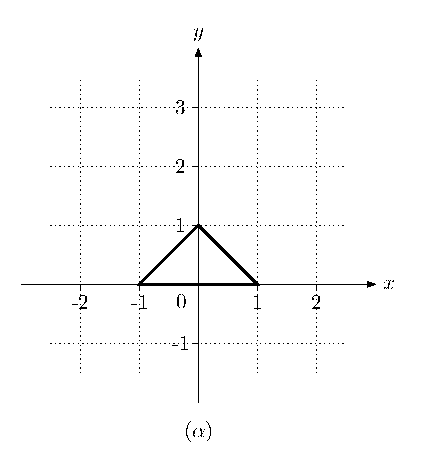
\includegraphics[width=\textwidth]{Chapter2/figure18a.pdf}
	\end{minipage}
\hfill
	\begin{minipage}[b]{0.3\textwidth} 
	    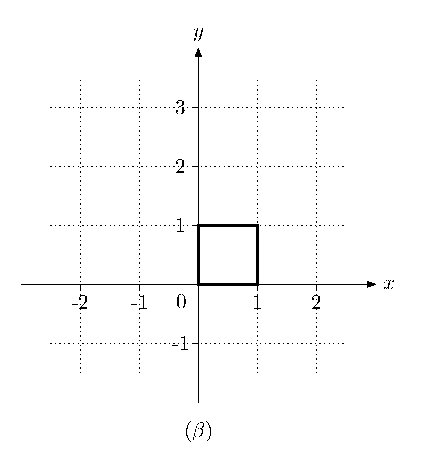
\includegraphics[width=\textwidth]{Chapter2/figure18b.pdf}
	\end{minipage}
\hfill
	\begin{minipage}[b]{0.3\textwidth} 
	    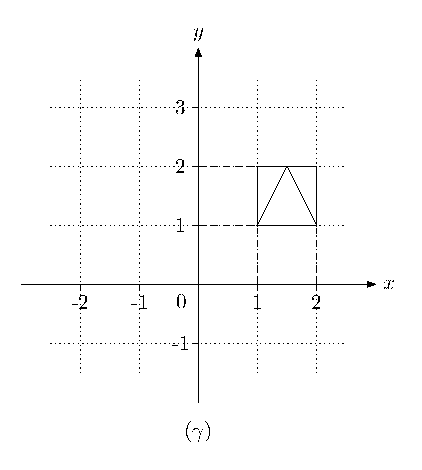
\includegraphics[width=\textwidth]{Chapter2/figure18c.pdf}
	\end{minipage}
\end{center}
\end{figure}

\end{exercise}

\begin{solution}
Πρώτα στην εικόνα (α) μπορούμε να δράσουμε ως εξής:
\begin{enumerate}
    \item Σύμπτυξη στις $x$-συντεταγμένες με: \(s_x = \cfrac{1}{2}\), \(s_y = 1\) (ως προς την αρχή των αξόνων).
    \item Μεταφορά κατά \(\vec{v} = (\cfrac{3}{2},1) \).
\end{enumerate}

Έτσι, παίρνουμε τον πίνακα μετασχηματισμού:
\[
M_{(a)} = T_v \cdot S_{\cfrac{1}{2},1} = \begin{bmatrix}
1 & 0 & \cfrac{3}{2} \\
0 & 1 & 1 \\
0 & 0 & 1
\end{bmatrix}
\begin{bmatrix}
\cfrac{1}{2} & 0 & 0 \\
0 & 1 & 0 \\
0 & 0 & 1
\end{bmatrix} = \begin{bmatrix}
\cfrac{1}{2} & 0 & \cfrac{3}{2} \\
0 & 1 & 1 \\
0 & 0 & 1
\end{bmatrix}
\]

Πράξεις:
\[
\begin{bmatrix}
\cfrac{1}{2} & 0 & \cfrac{3}{2} \\
0 & 1 & 1 \\
0 & 0 & 1
\end{bmatrix}
\begin{bmatrix}
-1 & 1 & 0 \\
0 & 0 & 1 \\
1 & 1 & 1
\end{bmatrix} = \begin{bmatrix}
1 & 2 & \cfrac{3}{2} \\
1 & 1 & 2 \\
1 & 1 & 1
\end{bmatrix}
\]


Αν στην εικόνα (β) μεταφερθεί κατά \(\vec{v} = (1,1)\), θα πάρουμε το τετράγωνο της εικόνας (γ):
\[
\begin{bmatrix}
1 & 0 & 1 \\
0 & 1 & 1 \\
0 & 0 & 1
\end{bmatrix}
\begin{bmatrix}
0 & 1 & 1 & 0 \\
1 & 0 & 1 & 1 \\
1 & 1 & 1 & 1
\end{bmatrix} = \begin{bmatrix}
1 & 2 & 2 & 1 \\
2 & 1 & 2 & 2 \\
1 & 1 & 1 & 1
\end{bmatrix}
\]

\end{solution}
